\section{Evaluation}\label{sec:eval}

To evaluate our approach, we set up two research questions as follows.

\begin{itemize}
\item RQ1. (Correctness) Does the transformation rules 
correctly transform single-GPU based model codes into
the distributed model codes?

\item RQ2. (Effectiveness) Does the automatic transformation result in speed-up 
in distributed training compared to single-GPU training?
\end{itemize}

To answer these questions, we implemented an automated code transformation tool
for TensorFlow DL model and experimented the tool against open-source
TensorFlow DL models. The code transformation tool is written in Scala and
is available at https://github.com/kaist-plrg/python-analyzer.
For experiment target models, we gathered open-source TensorFlow DL model
codes from three sources.
The Hovorod library GitHub repository\cite{horovodgithub} provides
example model codes. The TensorFlow model garden\cite{tfmodelgarden} is one of
the official collections of TensorFlow machine learning models. 
TensorFlow Examples by Americ Damien\cite{tfexmaplesdamien},
CIFAR-10 Example with TensorFlow 2.0\cite{cifar10github}, and
TensorFlow 2.x Tutorials\cite{tf2tutogithub} are popular GitHub repositories
that contain TensorFlow DL model codes.
Among these sources, we collected total of 16 models that are eligible
for the experiment.
The experiment target models are listed in figure \ref{fig:eval:targets}. 


%%%%%%%%%%%%%%%%%%%%%%%%%%%%
\pagebreak
\begin{figure}[!ht]
  \begin{center}
  \begin{tabular}{c|c|l}
    \hline
    Model Name & API Pattern & Source \\
    \hline
    LSTM-MNIST & GradientTape & \multirow{2}{*}{TensorFlow Examples by Americ Damien\cite{tfexamplesdamien}} \\
    SimpleCNN-GradientTape-1 & GradientTape \\
    \hline
    SimpleCNN-GradientTape-2 & GradientTape & \multirow{2}{*}{Horovod GitHub\cite{horovodgithub}} \\
    SimpleCNN-MonitoredSession & MonitoredSession  \\
    \hline
    SimpleCNN-Session & Session & TensorFlow Model Garden\cite{tfmodelgarden} \\
    \hline
    VGG-CIFAR10 & Keras & CIFAR-10 Example with TensorFlow 2.0\cite{cifar10github} \\
    \hline
    Play-with-MNIST & GradientTape & \multirow{10}{*}{TensorFlow 2.x Tutorials\cite{tf2tutogithub}} \\
    Linear-Regression & GradientTape  \\
    Fashion-MNIST & Keras  \\
    CIFAR10-VGG16 & GradientTape \\
    Inception-Network & GradientTape  \\
    RNN-Sentiment-Analysis & Keras  \\
    Stacked-LSTM-ColorBot & GradientTape  \\
    Auto-Encoder & GradientTape  \\
    Variational-Auto-Encoder & GradientTape  \\
    DCGAN & GradientTape  \\
    \hline
  \end{tabular}
  \end{center}
  \caption{List of the TensorFlow DL models used for the experiments}
  \label{fig:eval:targets}
\end{figure}


\subsection{RQ1: Transformation Experiment}

To answer the first research question,
we conducted a transformation experiment.
The transformation experiment evaluates whether the transformation tool
correctly transforms single-GPU based models to distributed models.
We specify the correctness of transfomation by pairing each model codes 
with hand-crafted code of the distributed versions. 
The models from the Horovod GitHub repository\cite{horovodgithub}
come with corresponding distributed versions.
For other models that do not come with distributed versions,
we manually crafted their distributed implmentations.

\begin{figure}[!ht]
  \begin{center}
  \begin{tabular}{|c|c|c|}
    \hline
    Model Name & API Pattern & Transformation Success \\
    \hline
    LSTM-MNIST & GradientTape & o \\
    SimpleCNN-GradientTape-1 & GradientTape & x\\
    SimpleCNN-GradientTape-2 & GradientTape & o \\
    SimpleCNN-MonitoredSession & MonitoredSession &o\\
    SimpleCNN-Session & Session & o\\
    VGG-CIFAR10 & Keras & o \\ 
    Play-with-MNIST & GradientTape & o \\
    Linear-Regression & GradientTape & o \\
    Fashion-MNIST & Keras & o \\
    CIFAR10-VGG16 & GradientTape & o\\
    Inception-Network & GradientTape & o \\
    RNN-Sentiment-Analysis & Keras & o \\
    Stacked-LSTM-ColorBot & GradientTape & o \\
    Auto-Encoder & GradientTape & o \\
    Variational-Auto-Encoder & GradientTape & o \\
    DCGAN & GradientTape & o \\
    \hline
  \end{tabular}
  \end{center}
  \caption{Transformation experiment Result}
  \label{fig:eval:trans}
\end{figure}

\begin{figure}[!ht]
  \begin{lstlisting}[language=Python]
# Model object is not used, instead a function used
def conv_net(x):
    x = tf.reshape(x, [-1, 28, 28, 1])
    conv1 = conv2d(x, weights['wc1'], biases['bc1'])
    conv1 = maxpool2d(conv1, k=2)
    conv2 = conv2d(conv1, weights['wc2'], biases['bc2'])
    conv2 = maxpool2d(conv2, k=2)
    fc1 = tf.reshape(conv2, [-1, weights['wd1'].get_shape().as_list()[0]])
    fc1 = tf.add(tf.matmul(fc1, weights['wd1']), biases['bd1'])
    fc1 = tf.nn.relu(fc1)
    out = tf.add(tf.matmul(fc1, weights['out']), biases['out'])
    return tf.nn.softmax(out)

optimizer = tf.optimizers.Adam(learning_rate)

def run_optimization(x, y):
    with tf.GradientTape() as g:
        pred = conv_net(x)
        loss = cross_entropy(pred, y) 
    trainable_variables = list(weights.values()) + list(biases.values())
    gradients = g.gradient(loss, trainable_variables)
    optimizer.apply_gradients(zip(gradients, trainable_variables))
    # cannot perform variable broadcast with Model.variables

# training loop
for step, (batch_x, batch_y) in enumerate(train_data.take(training_steps), 1):
    run_optimization(batch_x, batch_y)
  \end{lstlisting}
  \caption{Training code of SimpleCNN-GradientTape-1 model}
  \label{fig:eval:simplecnn1}
\end{figure}

The transformation experiment result is described in the 
figure \ref{fig:eval:trans}. Among 16 targets, only one model failed to
be correctly transformed. As shown in the figure \ref{fig:eval:trans},
the SimpleCNN-GradientTape-1 model failed to be transformed into the
distributed model.

We manually investigate the SimpleCNN-GradientTape-1 model code to 
identify the cause of the transformation failure.
The figure \ref{fig:eval:simplecnn1} illustrate the part of the training code
of the model.
The code uses the GradientTape pattern in lines 17 to 22, which
creates a {\tt GradientTape} object to record the computation
and automatically backpropagate the gradients to the model parameters.
It turns out that the code does not use the {\tt Model} instance to
define the neural network, instead define the function {\tt conv\_net} 
to eagerly compute the loss value.
To transform the GradientTape pattern codes into the distributed codes,
the vairable broadcast should be done to the {\tt variables} attributed of
the {\tt Model} instance. Because the SimpleCNN-GradientTape-1 training code
does not include the {\tt Model} instance, the code cannot be correctly
transformed into a distributed code by our transformation tool.
We argue that this is a very rare case, and our tool can transform most of the
codes. Among 11 target models of GraidentTape pattern, only
SimpleCNN-GradientTape-1 model fails to be correctly transformed.
All other model codes include the {\tt Model} instance, 
which is a common method to define the ML model in TensorFlow. 





\subsection{RQ2: Distributed Training Experiment}

To answer the second research question,
we conducted a distributed training experiment that compares
the training speed between the original models
and corresponding transform models.
To quantify the training speed, we measured the epoch loss during the training
of each model.
Among 16 models used for the first experiment,
we excluded two TensorFlow 1.x models (SimpleCNN-MonitoredSession,
SimpleCNN-Session) and the SimpleCNN-GradientTape-1 model that failed to
correctly be transformed.
Thus, we targeted total 13 models for the distributed training experiment.
We manually added the TensorBoard\cite{tensorboard} APIs to 
record the loss value during the training. 
The experiment server uses
Intel Xeon CPU E5-2690 v4 @ 2.60GHz with 131GB memory and four 
NVIDIA TITAN Xp GPUs.

\begin{figure}[!ht]
  \centering
  \begin{subfigure}[t]{.24\textwidth}
    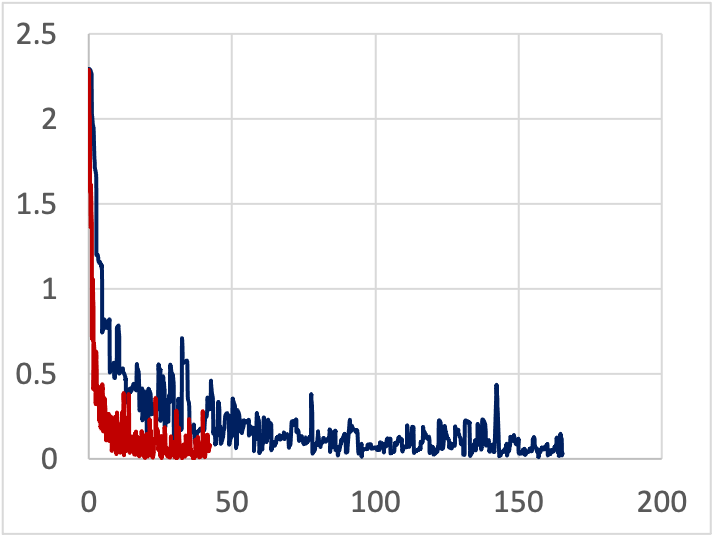
\includegraphics[width=\textwidth]{tape-lstm}
    \caption{LSTM-MNIST}
  \end{subfigure}
  ~ 
  \begin{subfigure}[t]{.24\textwidth}
    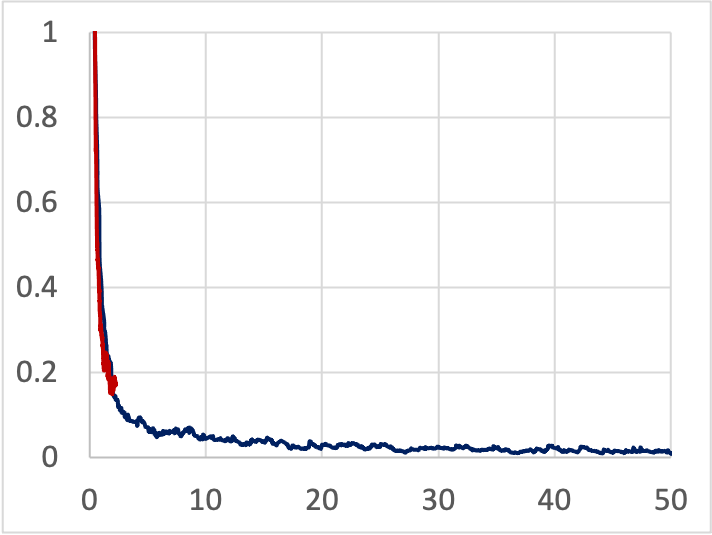
\includegraphics[width=\textwidth]{tape-simple2}
    \caption{SimpleCNN-GradientTape-2}
  \end{subfigure}
  ~
  \begin{subfigure}[t]{.24\textwidth}
    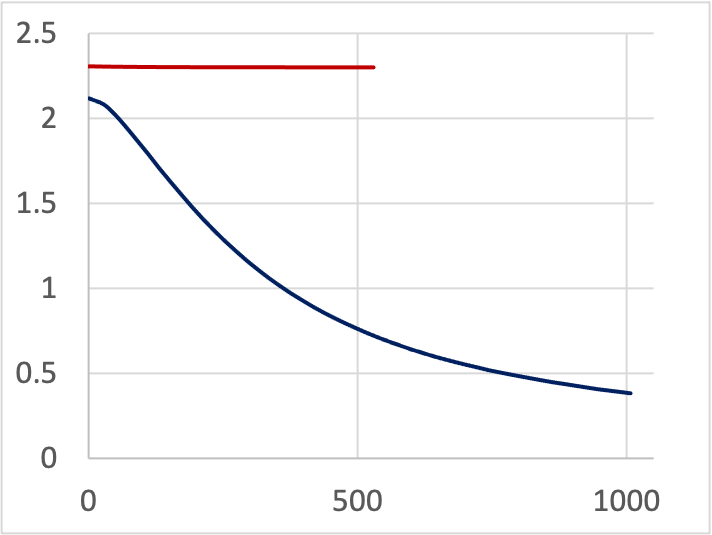
\includegraphics[width=\textwidth]{keras-cifar}
    \caption{VGG-CIFAR10}
  \end{subfigure}
  \par\bigskip
  \begin{subfigure}[t]{.24\textwidth}
    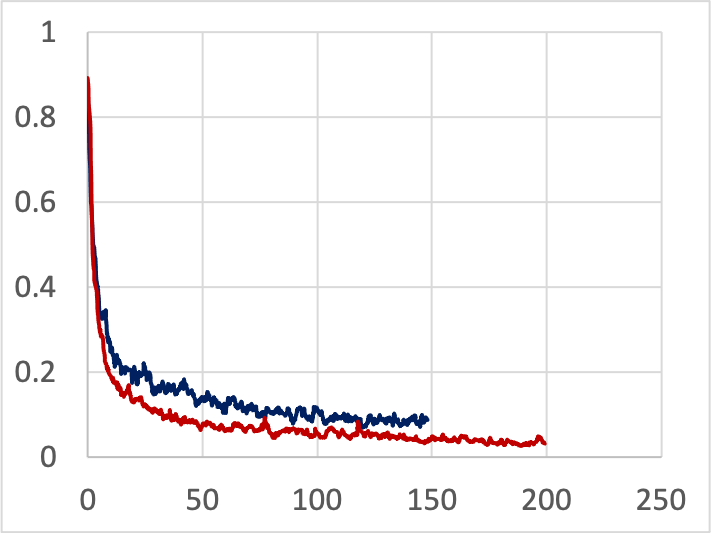
\includegraphics[width=\textwidth]{tf2-03}
    \caption{Play-with-MNIST}
  \end{subfigure}
  ~
  \begin{subfigure}[t]{.24\textwidth}
    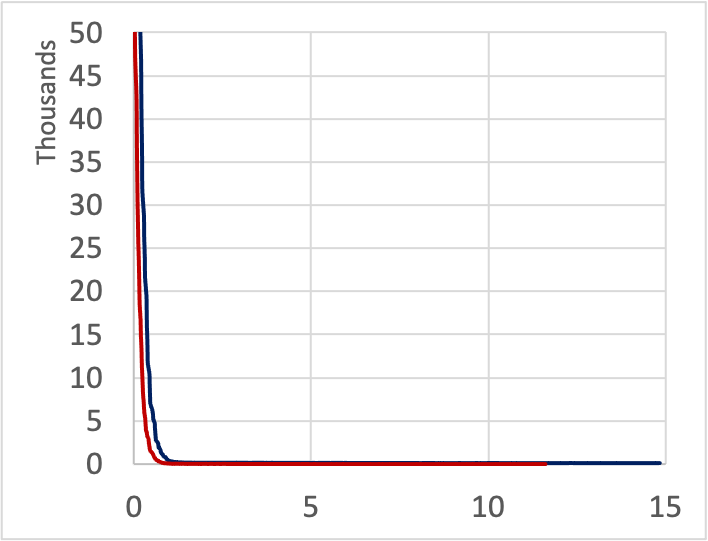
\includegraphics[width=\textwidth]{tf2-04}
    \caption{Linear-Regression}
  \end{subfigure} 
  ~ 
  \begin{subfigure}[t]{.24\textwidth}
    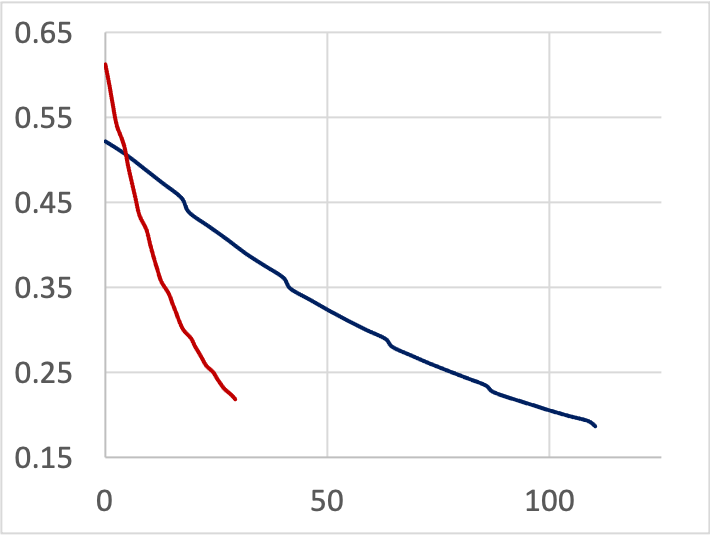
\includegraphics[width=\textwidth]{tf2-05}
    \caption{Fashion-MNIST}
  \end{subfigure}
  ~
  \begin{subfigure}[t]{.24\textwidth}
    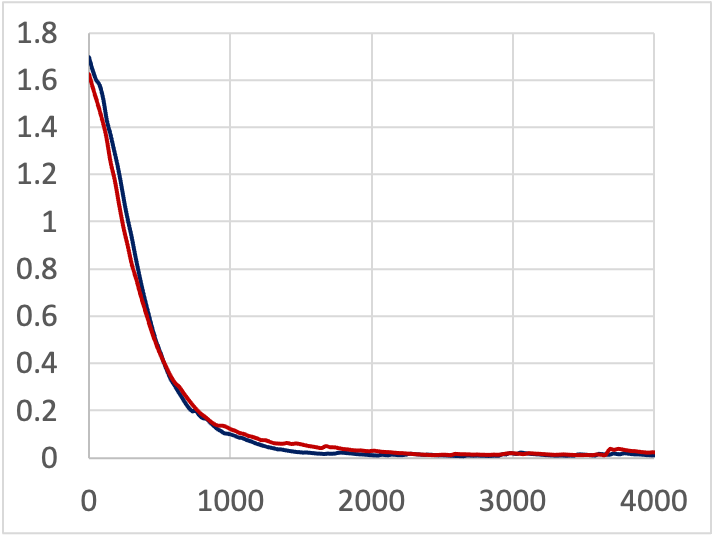
\includegraphics[width=\textwidth]{tf2-06}
    \caption{CIFAR10-VGG16}
  \end{subfigure}
  \par\bigskip
  \begin{subfigure}[t]{.24\textwidth}
    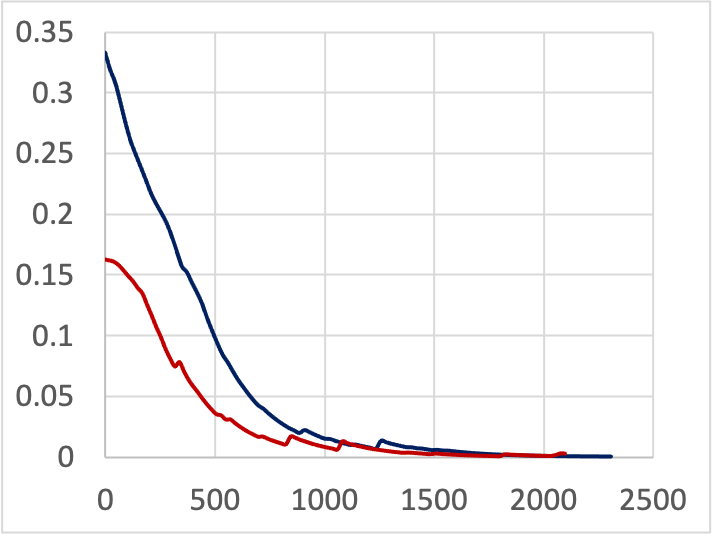
\includegraphics[width=\textwidth]{tf2-07}
    \caption{Inception-network}
  \end{subfigure}
  ~
  \begin{subfigure}[t]{.24\textwidth}
    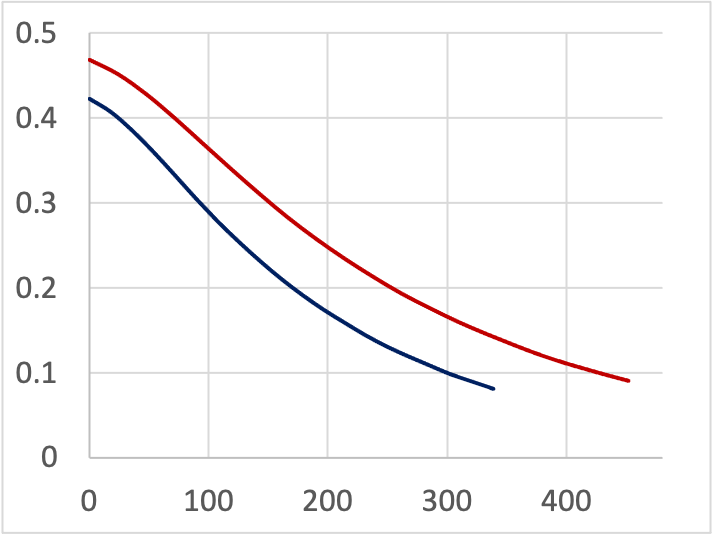
\includegraphics[width=\textwidth]{tf2-09}
    \caption{RNN-Sentiment-Analysis}
  \end{subfigure} 
  ~ 
  \begin{subfigure}[t]{.24\textwidth}
    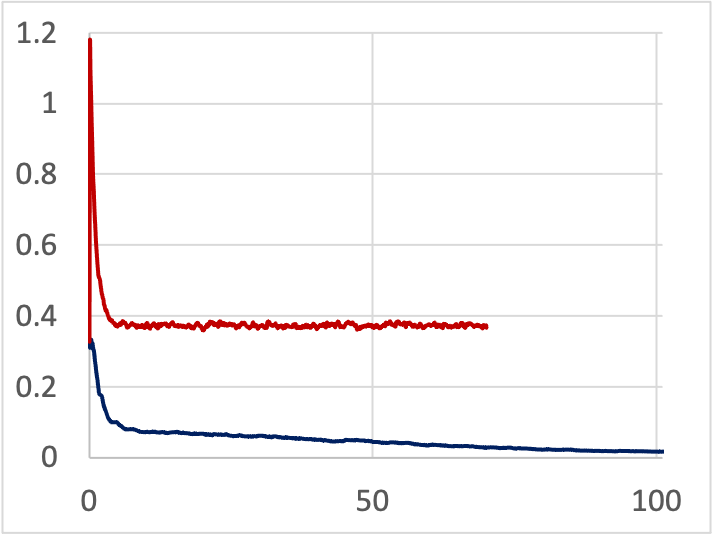
\includegraphics[width=\textwidth]{tf2-10}
    \caption{Stacked-LSTM-ColorBot}
  \end{subfigure}
  ~
  \begin{subfigure}[t]{.24\textwidth}
    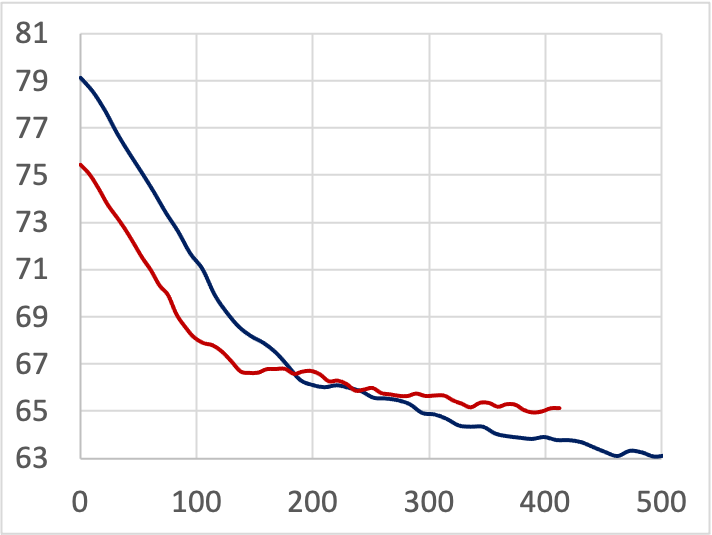
\includegraphics[width=\textwidth]{tf2-11}
    \caption{Auto-Encoder}
  \end{subfigure}
  \par\bigskip
  \begin{subfigure}[t]{.24\textwidth}
    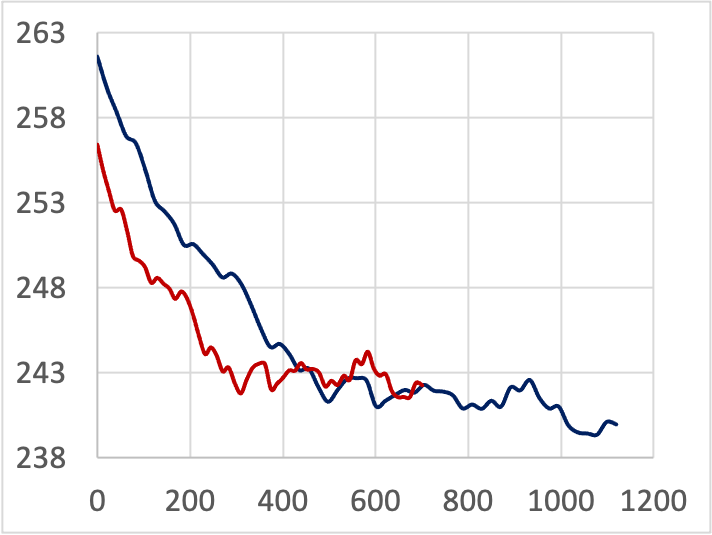
\includegraphics[width=\textwidth]{tf2-12}
    \caption{Variational-Auto-Encoder}
  \end{subfigure}
  ~
  \begin{subfigure}[t]{.24\textwidth}
    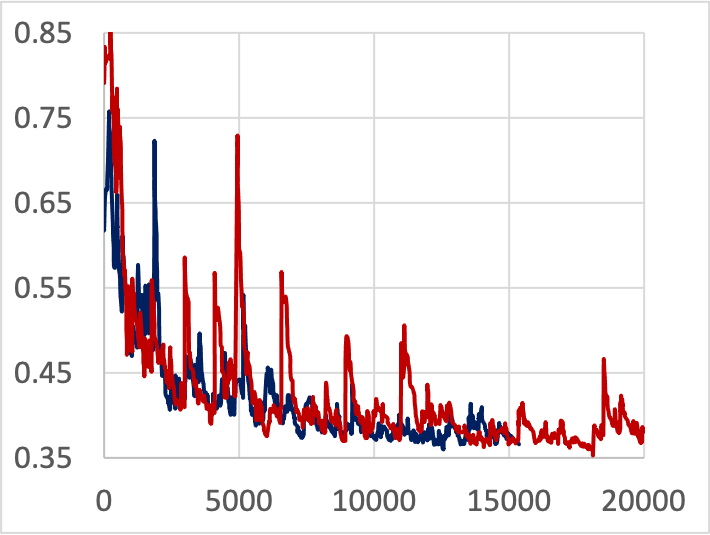
\includegraphics[width=\textwidth]{tf2-13}
    \caption{DCGAN}
  \end{subfigure} 

  \caption{Distributed training experiment result time-loss graphs.}
  \begin{tabular}{r@{: }l r@{: }l}
    X-axis & Time (seconds) & Y-axis & Loss value\\
    Blue line & ORG loss, smoothed & Red line & HVD loss, smoothed\\ 
  \end{tabular}
  \label{fig:eval:train}
\end{figure}


\begin{figure}
  \centering
  \begin{tabular}{|l|r|r|r|}
\hline
                         & Single-GPU         & Distributed       & \\
Model Name               &  training time (s) & training time (s) &  Speedup\\
\hline
LSTM-MNIST               & 78.675& 11.951& $\times$6.58\\
SimpleCNN-GradientTape-2 & 3.192& 1.753& $\times$1.82\\
VGG-CIFAR10              & 1060.296  & 1159.293  &$\times$0.91   \\
Play-with-MNIST          & 148.101& 80.040& $\times$1.85\\
Linear-Regression        & 0.607& 0.371& $\times$1.63\\
Fashion-MNIST            & 110.274& 29.294& $\times$3.76\\
CIFAR10-VGG16            & 1060.296& 1159.293& $\times$0.91\\
Inception-network        & 956.261& 995.597& $\times$0.96\\
RNN-Sentiment-Analysis   & 338.984& 451.985& $\times$0.74\\
Stacked-LSTM-ColorBot    & 57.327 & -           & -   \\
Auto-Encoder             & 567.230& 412.214& $\times$1.37\\
Variational-Auto-Encoder & 1120.291& 699.777& $\times$1.60\\
DCGAN                    & 2389.052& 828.428& $\times$2.88\\ 
\hline
  \end{tabular}
  \caption{Training time and speedup between single GPU-based models and automatically transformed distributed models}
  \label{fig:eval:traintime}
\end{figure}

The results of the distributed traininig experiment 
are shown in figure \ref{fig:eval:train} and figure \ref{fig:eval:traintime}.
Figure \ref{fig:eval:train} graphically describes the change of training loss
of single GPU-based models and distributed models over time.
The x-axis represent the time in seconds, and the y-axis represent
the loss value number.
The lines represent the loss values;
blue lines correspond to the single GPU-based model training loss
and the red lines correspond to the distributed model training loss.
Figure \ref{fig:eval:traintime} show the training times required in
single GPU-based models and distributed models.
To define the training time, we first calculated the total reduction of
loss by finding the maximum and minimum losses.
We define that the training has completed when the loss decreased by
95\% of the loss reduction amount, and the time up to that point
was defined as the training time.
The fourth column of figure \ref{fig:eval:traintime} 
shows the relative speedup of the 
distributed model training with respect to the single GPU-based model training.
Note that the Stacked-LSTM-ColorBot model does not have distributed training
time recorded. This is because the loss values after the first epoch
are always higher that the initial loss value; thus the training time is
undefined.

As shown in the results in figure \ref{fig:eval:traintime},
only 8 out of 13 distributed models show speedup. 
Figure \ref{fig:eval:train} also shows that some models are erroneously trained.
In figure \ref{fig:eval:train}(c), the distributed training of
VGG-CIFAR10 model does not decrease the loss value.
In figure \ref{fig:eval:train}(j), the distributed training of
Stacked-LSTM-ColorBot model increases the loss value.
In general, the experiment result implies that even if the transformation
of the model code is successful, it does not guarantee
increase in the training speed of the distributed models.

We claim that training hyperparameters can be tuned to
achieve the distributed training speedup.
We provide an experimental evidence to this by
training the distributed VGG-CIFAR10 model with
different learning rates.
Learning rate value of the original VGG-CIFAR10 model is 0.001.
We altered this value to 0.0001, 0.00001, and 0.000001
and compared the training loss changes over time.

\begin{figure}[!ht]
  \centering
  \begin{subfigure}[t]{.24\textwidth}
    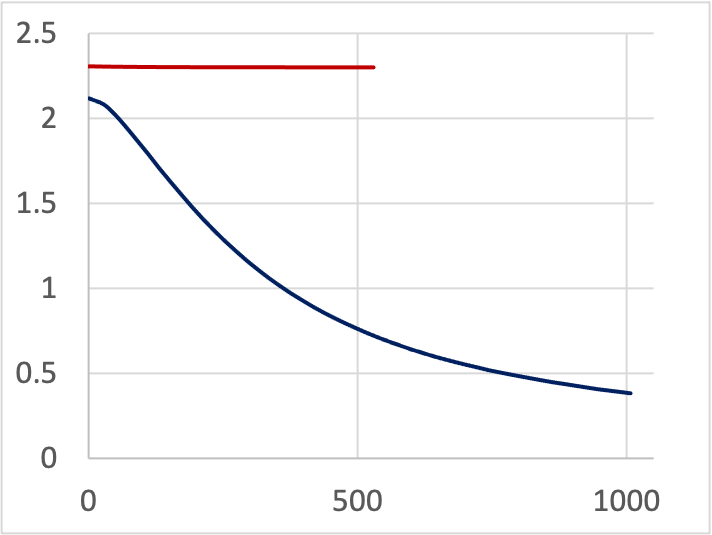
\includegraphics[width=\textwidth]{keras-cifar}
    \caption{VGG-CIFAR10 model with lr=0.001 (default value)}
  \end{subfigure}
  ~
  \begin{subfigure}[t]{.24\textwidth}
    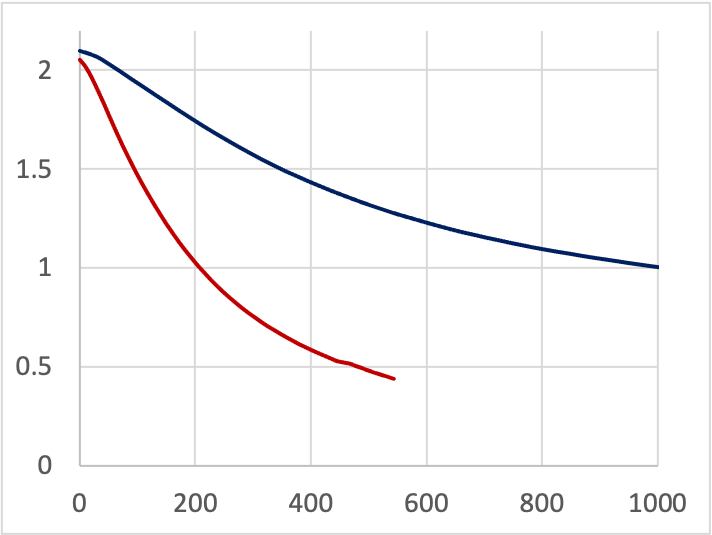
\includegraphics[width=\textwidth]{cifar-1e4}
    \caption{VGG-CIFAR10 model with lr=0.0001}
  \end{subfigure} 
  ~ 
  \begin{subfigure}[t]{.24\textwidth}
    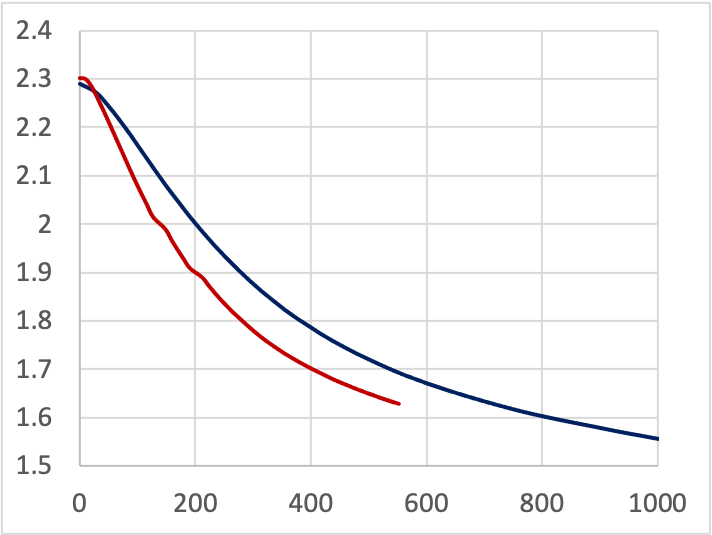
\includegraphics[width=\textwidth]{cifar-1e5}
    \caption{VGG-CIFAR10 model with lr=0.00001}
  \end{subfigure}
  ~
  \begin{subfigure}[t]{.24\textwidth}
    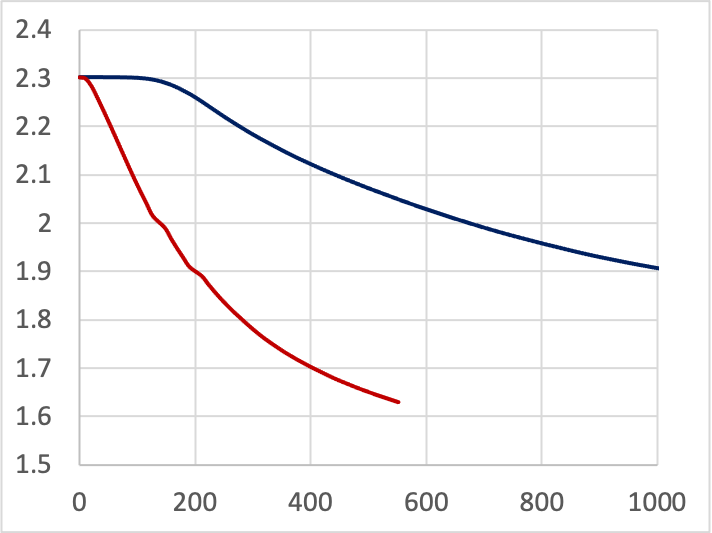
\includegraphics[width=\textwidth]{cifar-1e6}
    \caption{VGG-CIFAR10 model with lr=0.000001}
  \end{subfigure}

  \caption{Distributed training experiments of VGG-CIFAR10 model with different learning rates.}
  \begin{tabular}{r@{: }l r@{: }l}
    X-axis & Time (seconds) & Y-axis & Loss value\\
    Blue line & ORG loss, smoothed & Red line & HVD loss, smoothed\\ 
  \end{tabular}
  \label{fig:eval:cifar10}
\end{figure}

Figure \ref{fig:Eval:cifar10} shows the loss value changes of training 
distributed VGG-CIFAR10 models with different learning rates.

The results show that the training speed difference between single-GPU and
distributed training can differ according to the model hyperparameters
such as the learning rate. The fact that various combinations of hyperparameters
must be considered and experiement to reach optimal training speed is 
well-known in ML community. This problem also applies to distributed training,
where optimial hyperparameters should be re-searched after the training
code is transformed. Our transformation tool do not target to search the 
optimal hyperparameters, although we do implement the guidelines from the
official Horovod documents to scale learning rate and epoch numbers
by number of the GPUs.  

Although the automatically transformed model codes may need additional
tuning, our transformation tool effectively reduces
burdens of manually rewriting the training codes.
By applying our tool, the users can quickly change the single-GPU-based
models into the distributed model and initiate the tranining.
During the training process, the user may monitor training-related measurements
such as per-epoch loss and decide to tune the hyperparameters.
From the transformed training code, the user is able to quickly locate the
hyperparameter variables, which suffer none-or-minimal changes of their locations
from the original code.
Therefore, the users of our tool can quickly iterate the process of
training, evaluating and tuning without rewriting the
training code with manual investigation on the library documentations and
the model code.
